\documentclass[11pt,a4paper]{article}

\usepackage[margin=0.78in]{geometry}
\usepackage[T1]{fontenc}
\usepackage{lmodern}
\usepackage{microtype}
\usepackage{xcolor}
\usepackage{graphicx}
\usepackage{array}
\usepackage{booktabs}
\usepackage{tabularx}
\usepackage{enumitem}
\usepackage{listings}
\usepackage{fancyhdr}
\usepackage{hyperref}
\usepackage{float}
\usepackage{tikz}
\usetikzlibrary{arrows.meta,backgrounds}

\definecolor{forest}{HTML}{28523A}
\definecolor{soft}{HTML}{F1F5EF}
\definecolor{muted}{HTML}{5B685F}

\hypersetup{
  colorlinks=true,
  linkcolor=forest,
  urlcolor=forest,
  pdftitle={Calculator REST API DevOps Project Report},
  pdfauthor={Manzil Baruah}
}

\pagestyle{fancy}
\fancyhf{}
\lhead{SPE Mini Project}
\rhead{Calculator REST API and DevOps}
\cfoot{\thepage}
\setlength{\headheight}{14pt}

\lstdefinestyle{code}{
  basicstyle=\ttfamily\footnotesize,
  breaklines=true,
  frame=single,
  rulecolor=\color{forest!35},
  backgroundcolor=\color{soft},
  showstringspaces=false,
  columns=fullflexible,
  keepspaces=true,
  xleftmargin=4pt,
  xrightmargin=4pt,
  aboveskip=7pt,
  belowskip=7pt
}
\lstset{style=code}
\newcolumntype{Y}{>{\raggedright\arraybackslash}X}

\newcommand{\screenshotplaceholder}[2]{%
  \begin{figure}[H]
    \centering
    \fbox{\parbox[c][1.15in][c]{0.91\linewidth}{\centering
      {\large\bfseries Screenshot placeholder: #1}\\[6pt]
      {\small #2}\\[5pt]
      {\footnotesize Replace this box with the requested screenshot before submission.}}}
    \caption{#1}
  \end{figure}
}

\title{\textbf{Calculator REST API\\DevOps Project Report}}
\author{Manzil Baruah\\Roll Number: MT2025715}
\date{30 October 2026}

\begin{document}
\maketitle
\begin{center}
\textbf{Course:} CSE 816 -- Software Production Engineering\\
\textbf{Project:} End-to-End CI/CD Pipeline for a Calculator REST API\\
\textbf{Repository:} \url{https://github.com/certifiedUnc/SPE_Mini_Project-main}\\
\textbf{Target image:} \texttt{certifiedunc/spe-calculator}
\end{center}

\section{Introduction: What and Why of DevOps?}
DevOps combines software development and IT operations practices so teams can build, test, package, and deliver software through repeatable steps and timely feedback. Source control, automated testing, container images, and deployment automation reduce manual handoffs and make changes easier to review and reproduce.

This project applies those ideas to a calculator service. It provides a Java 21 and Spring Boot REST API with a browser interface. Maven runs the tests and packages the application. Docker creates a multi-stage application image, while Docker Compose starts the calculator alongside an Nginx reverse proxy. A declarative Jenkins pipeline defines validation, build, test, package, image, push, and deploy stages.

\begin{center}
\fcolorbox{forest}{soft}{\parbox{0.93\linewidth}{
\textbf{Project status.} The application, tests, Docker configuration, Compose stack, and Jenkins pipeline are present in the public repository. Local Maven verification and local service health/API checks have passed. Jenkins requires first-run administrator setup and account credentials before an end-to-end Jenkins build can be claimed.}}
\end{center}

\subsection{Architecture}
\begin{figure}[H]
\centering
\resizebox{\linewidth}{!}{%
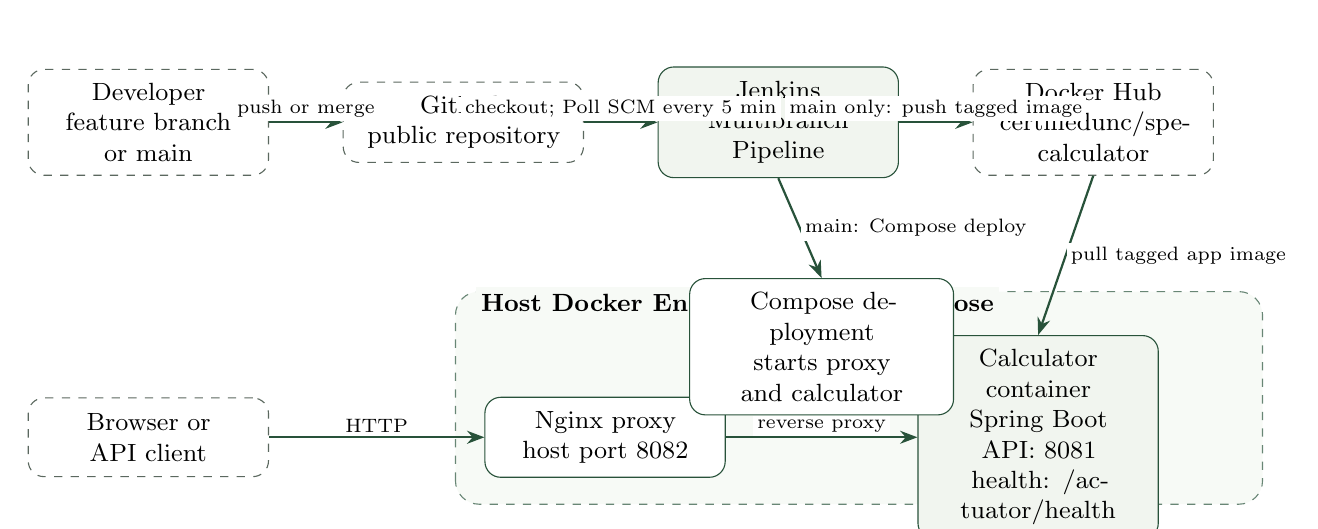
\begin{tikzpicture}[
  x=1cm,y=1cm,
  nodebox/.style={draw=forest,rounded corners=2mm,align=center,
    minimum width=2.8cm,minimum height=1.0cm,text width=2.7cm,
    font=\small,inner sep=5pt,fill=white},
  external/.style={nodebox,dashed,draw=muted},
  flow/.style={-{Stealth[length=2.2mm]},draw=forest,thick},
  flowlabel/.style={font=\scriptsize,fill=white,inner sep=1.5pt,align=center}
]
  % CI/CD flow
  \node[external] (developer) at (0,4) {Developer\\feature branch or main};
  \node[external] (github) at (4,4) {GitHub\\public repository};
  \node[nodebox,fill=soft] (jenkins) at (8,4) {Jenkins\\Multibranch Pipeline};
  \node[external] (hub) at (12,4) {Docker Hub\\certifiedunc/spe-calculator};

  \draw[flow] (developer.east) -- node[flowlabel,above] {push or merge} (github.west);
  \draw[flow] (github.east) -- node[flowlabel,above] {checkout; Poll SCM every 5 min} (jenkins.west);
  \draw[flow] (jenkins.east) -- node[flowlabel,above] {main only: push tagged image} (hub.west);

  % Runtime and deployment host
  \begin{scope}[on background layer]
    \draw[rounded corners=3mm,dashed,draw=forest!70,fill=soft!55]
      (3.9,-0.85) rectangle (14.15,1.85);
  \end{scope}
  \node[font=\small\bfseries,anchor=west,fill=soft!55,inner sep=2pt]
    at (4.15,1.68) {Host Docker Engine / Docker Compose};

  \node[external] (client) at (0,0) {Browser or API client};
  \node[nodebox] (proxy) at (5.8,0) {Nginx proxy\\host port 8082};
  \node[nodebox,fill=soft] (calculator) at (11.3,0)
    {Calculator container\\Spring Boot API: 8081\\health: /actuator/health};
  \node[nodebox,fill=white,minimum width=3.2cm,text width=3.0cm]
    (compose) at (8.55,1.15) {Compose deployment\\starts proxy and calculator};

  \draw[flow] (client.east) -- node[flowlabel,above] {HTTP} (proxy.west);
  \draw[flow] (proxy.east) -- node[flowlabel,above] {reverse proxy} (calculator.west);
  \draw[flow] (jenkins.south) -- node[flowlabel,right] {main: Compose deploy} (compose.north);
  \draw[flow] (hub.south) -- node[flowlabel,right] {pull tagged app image} (calculator.north);
\end{tikzpicture}%
}
\caption{CI/CD flow and runtime deployment architecture. The Jenkins pipeline pushes and deploys only from \texttt{main}; the local Jenkins setup uses polling until a public webhook URL is available.}
\end{figure}

\section{Tools Used}
\begin{enumerate}[leftmargin=*,itemsep=2pt]
  \item \textbf{Git and GitHub}: source control, public repository, feature branches, and merged changes.
  \item \textbf{Java 21 and Spring Boot}: REST API, static calculator interface, and Actuator health endpoint.
  \item \textbf{Maven}: dependency management, compilation, testing, and executable JAR packaging.
  \item \textbf{JUnit 5, Spring Boot Test, and MockMvc}: service unit tests and REST/controller integration tests.
  \item \textbf{Jenkins}: declarative, multibranch CI/CD pipeline with JUnit publication and email-extension hooks.
  \item \textbf{Docker}: multi-stage application image and container runtime.
  \item \textbf{Docker Compose}: calculator and proxy services, networks, health checks, and deployment.
  \item \textbf{Nginx}: reverse proxy for the browser interface and API.
  \item \textbf{Docker Hub}: target registry configured in the pipeline as \texttt{certifiedunc/spe-calculator}.
\end{enumerate}

\section{Step-by-Step Implementation}
\subsection{Step 1: Source Control Management (Git and GitHub)}
The repository is public and contains the application, build files, Docker configuration, Jenkinsfile, README, and project evidence. Work was committed in multiple changes. Feature branches were created and merged into \texttt{main}; the calculator UI branch is \texttt{feature/polished-calculator-ui}.

A Jenkins Multibranch Pipeline job can discover branches containing a Jenkinsfile. The repository's Jenkinsfile uses Poll SCM every five minutes once that job is configured, which provides a trigger even when a GitHub webhook cannot reach a local Jenkins installation. A webhook can be added when Jenkins has a publicly reachable URL.

\begin{lstlisting}
git switch main
git pull --ff-only origin main
git switch -c feature/describe-your-change
# make and review changes
git diff
git add <files>
git commit -m "Describe the change"
git push -u origin feature/describe-your-change
\end{lstlisting}

\screenshotplaceholder{GitHub repository and history}{Capture the public repository page, branch list, and meaningful commit/merge history.}

\subsection{Step 2: REST API and Functional Behavior}
The calculator accepts decimal values as query parameters and returns a JSON object containing the operation, both operands, and the result.

\begin{center}
\begin{tabularx}{\linewidth}{@{}l l Y@{}}
\toprule
\textbf{Operation} & \textbf{Endpoint} & \textbf{Behavior} \\
\midrule
Add & \texttt{GET /api/v1/add?a=2\&b=3} & Returns the sum. \\
Subtract & \texttt{GET /api/v1/subtract?a=7\&b=3} & Returns the difference. \\
Multiply & \texttt{GET /api/v1/multiply?a=2.5\&b=4} & Returns the product. \\
Divide & \texttt{GET /api/v1/divide?a=7\&b=2} & Returns the quotient; division by zero returns HTTP 400. \\
Health & \texttt{GET /actuator/health} & Spring Actuator reports application health. \\
\bottomrule
\end{tabularx}
\end{center}

Example successful response:
\begin{lstlisting}
{"operation":"add","a":2,"b":3,"result":5}
\end{lstlisting}

Missing parameters, non-numeric values, and division by zero return HTTP 400 with a structured JSON error containing an error code, message, and status. The health endpoint is used by the application container health check.

\subsection{Step 3: Automated Testing (JUnit 5 and MockMvc)}
The service tests cover addition, subtraction, multiplication, division, and division by zero. Spring MVC integration tests use MockMvc to call API endpoints and verify success responses and structured errors; they also verify that the calculator frontend is served.

Run the test suite locally with:
\begin{lstlisting}
mvn -B -ntp clean verify
\end{lstlisting}

The verified run completed 10 tests with zero failures and errors. Maven Surefire writes JUnit XML files under \texttt{target/surefire-reports/}; Jenkins publishes those reports through its JUnit step.

\screenshotplaceholder{Maven test results}{Capture the terminal output showing Maven build success and the test count, or Jenkins' published test report.}

\subsection{Step 4: Build and Continuous Integration (Jenkins)}
The declarative \texttt{Jenkinsfile} defines these stages:
\begin{enumerate}[leftmargin=*,itemsep=2pt]
  \item \textbf{Checkout}: checks out the exact repository revision for the branch.
  \item \textbf{Validate Compose}: runs \texttt{docker compose config --quiet}.
  \item \textbf{Build}: runs \texttt{mvn -B -ntp -DskipTests clean package}.
  \item \textbf{Test}: runs \texttt{mvn -B -ntp test}, publishes JUnit XML, and fails when tests fail.
  \item \textbf{Package}: archives the executable JAR in Jenkins.
  \item \textbf{Docker Build}: builds a branch/build-number tagged calculator image and the Nginx proxy image.
  \item \textbf{Push}: only on \texttt{main}, logs into Docker Hub using Jenkins-managed credentials and pushes a versioned tag and \texttt{latest}.
  \item \textbf{Deploy}: only on \texttt{main}, runs Docker Compose and waits for service health checks.
\end{enumerate}

Jenkins runs in Docker at \url{http://localhost:8090}. Its image contains Java 21, Maven, Docker CLI, Docker Compose v2, and the Git, Pipeline, GitHub Branch Source, Workspace Cleanup, JUnit, and Email Extension plugins. The Docker socket group ID is supplied through \texttt{DOCKER\_GID}. Docker Hub uses Jenkins credential ID \texttt{dockerhub-credentials}. Email actions target the configured student address and require SMTP settings in Jenkins.

\begin{center}
\fcolorbox{forest}{soft}{\parbox{0.93\linewidth}{
\textbf{External setup/evidence still required:} finish Jenkins first-run administrator setup; add Docker Hub credentials; configure SMTP if email delivery is required; create and scan the GitHub Multibranch Pipeline job; then run the \texttt{main} job. Poll SCM is enabled. No successful Jenkins push/deploy run is claimed in this report.}}
\end{center}

\screenshotplaceholder{Jenkins pipeline stages}{After the first successful main build, capture Stage View with Checkout, Validate Compose, Build, Test, Package, Docker Build, Push, and Deploy.}

\subsection{Step 5: Containerization (Docker)}
The application Dockerfile uses a Maven/Java 21 build stage and a Java 21 JRE runtime stage. Maven dependencies are cached during image construction. The runtime image copies only the packaged application JAR, creates and uses a non-root account, exposes port 8081, and defines a health check against \texttt{/actuator/health}. A \texttt{.dockerignore} excludes source-control metadata, build output, local configuration, and unrelated files from the Docker build context.

Build and run a local image directly:
\begin{lstlisting}
docker build -t local/spe-calculator:dev .
docker run --rm --name spe-calculator -p 8081:8081 local/spe-calculator:dev
\end{lstlisting}

\screenshotplaceholder{Docker image or running container}{Capture the image build and container status, including the mapped application port.}

\subsection{Step 6: Deployment and Orchestration (Docker Compose and Nginx)}
The Compose stack contains two services. The calculator is attached to an internal network and is not published directly to the host. Nginx is connected to the calculator network and a proxy network, and publishes port 8082 to the host. Both services have health checks and restart policies. The calculator also runs read-only with a temporary writable directory, dropped Linux capabilities, and no-new-privileges enabled.

Start and verify the full stack:
\begin{lstlisting}
docker compose up -d --build --wait --wait-timeout 120
docker compose ps
curl --fail http://localhost:8082/actuator/health
curl --fail 'http://localhost:8082/api/v1/add?a=2&b=3'
\end{lstlisting}

The local check returned \texttt{UP} for the health endpoint and a result of 5 for the sample addition. The browser calculator is available at \url{http://localhost:8082}. The proxy port can be overridden with \texttt{PROXY\_PORT} when 8082 is already occupied.

\screenshotplaceholder{Compose services and health checks}{Capture \texttt{docker compose ps} with both services healthy and terminal health/API responses.}
\screenshotplaceholder{Calculator user interface}{Capture the calculator page showing the current interface, including the Clear control and result panel.}

\section{Results, Challenges, and Remaining Evidence}
The application, its unit and MVC tests, the multi-stage container build, and the two-service Compose deployment are implemented. The current GitHub \texttt{main} branch includes a feature branch merge and a separate Jenkins pipeline update that introduced the explicit Build stage. Local Maven verification and local API/health checks have been run successfully.

The Jenkins image and plugins are prepared locally, and the Jenkins container has Docker socket access. However, Jenkins still requires first-run administrator setup, Docker Hub credentials, and (if email evidence is required) SMTP configuration. A GitHub webhook is not configured because this Jenkins instance is local-only; the pipeline's five-minute polling trigger is enabled instead. Capture Jenkins and Docker Hub screenshots only after those external steps and a successful pipeline run.

\begin{center}
\fcolorbox{forest}{soft}{\parbox{0.93\linewidth}{
\textbf{Submission checklist:} replace each screenshot placeholder; run \texttt{mvn clean verify}; complete Jenkins setup and configure its credentials; run the \texttt{main} pipeline; verify the pushed Docker Hub tag and deployed Compose health; and attach email evidence if SMTP delivery is part of the assessment.}}
\end{center}

\screenshotplaceholder{Docker Hub image tags}{After a successful authenticated pipeline push, capture the repository page showing the build-specific image tag and \texttt{latest}.}
\screenshotplaceholder{Build status email}{If SMTP is configured, capture the Jenkins success email in the recipient inbox.}

\end{document}
